% 图 64.1 —— 由 `checks/emit_hand.py` 自动拼出（probe 精测 + prims2 图元分解）
%%
% ⚠ 这是**稿子不是成品**：跑 `checks/checkhand.py 64.1` 看指标 + 看叠合图。
%%
%% ⚠ 待核：
%   · 本图 probe 报出阴影族 1 个 —— **本脚本不生成阴影**（要照原书手写）；prims2 的 strokes 里可能含阴影线，核对时留意别画重
%   · 可疑字形 1 项（空心圈 ⊙ 常被认成字母 o）—— 见文件末
%%
\documentclass[12pt]{standalone}
\usepackage{fontspec}
\setsansfont{Arial}
\newfontfamily\mfallback{DejaVu Sans}
\usepackage{tikz}
\begin{document}
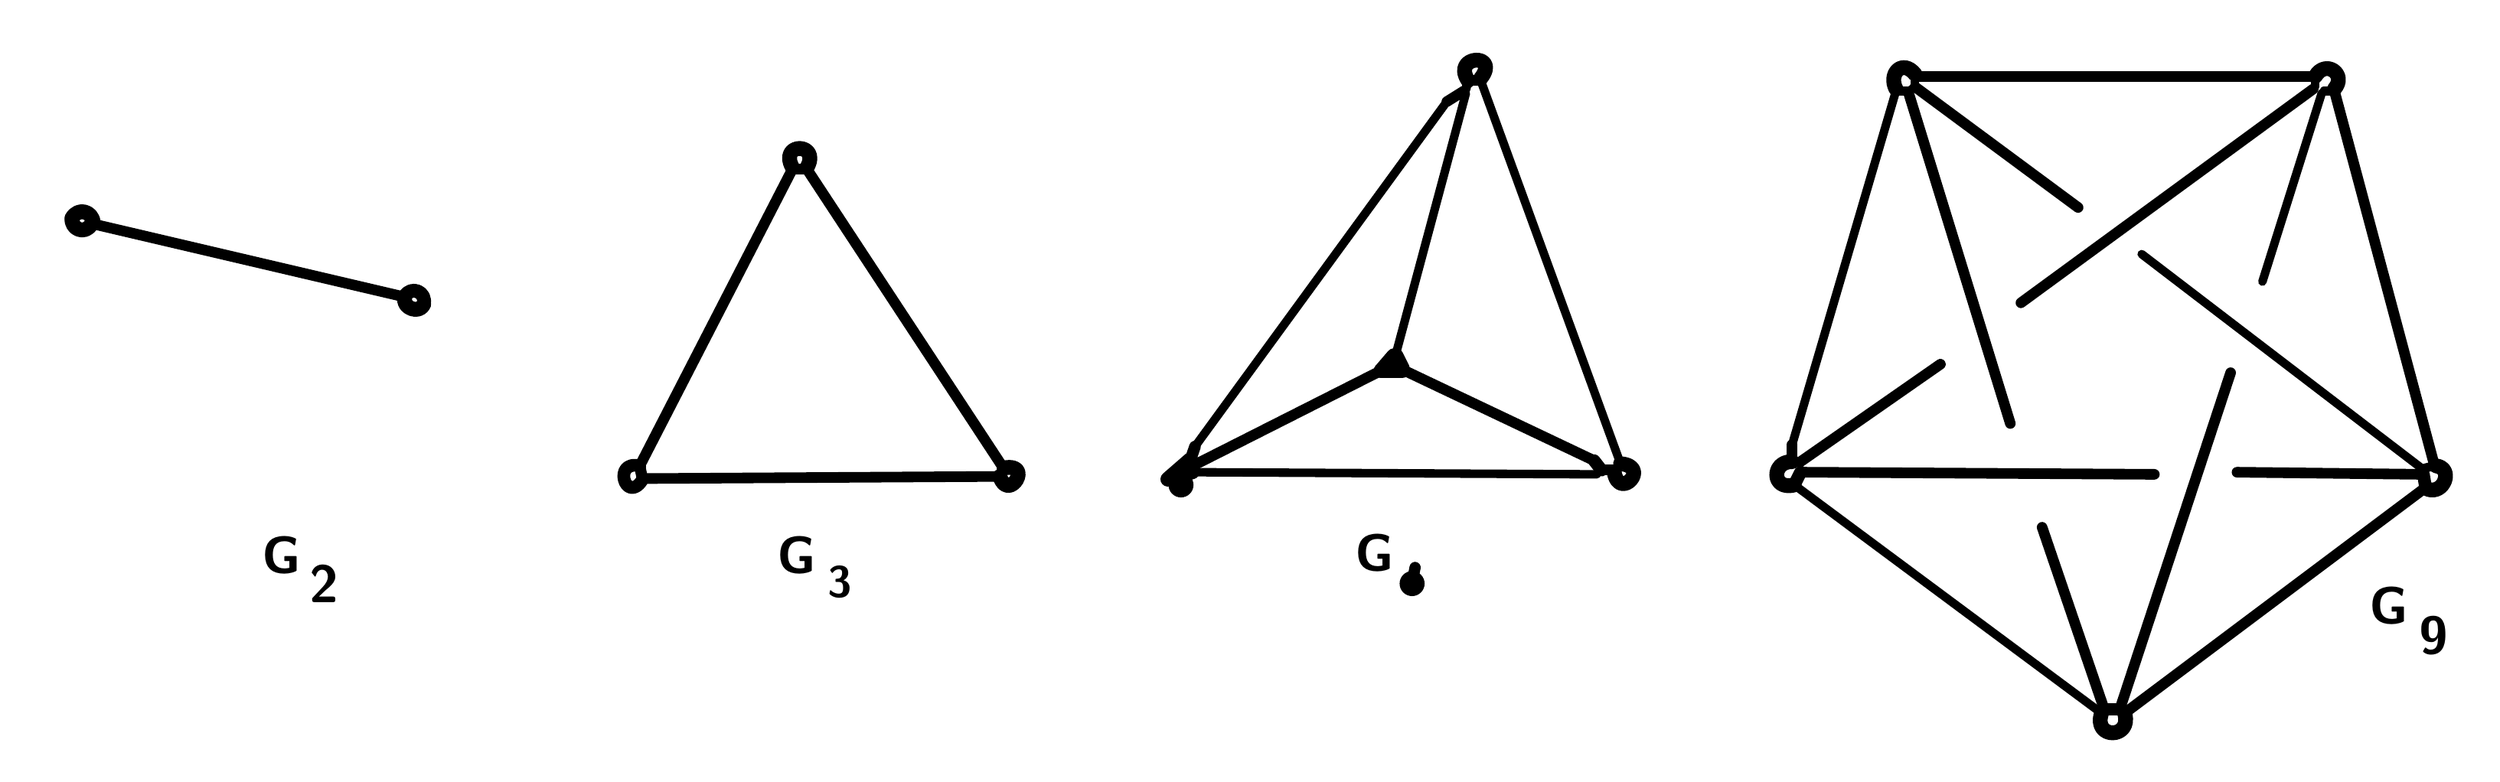
\begin{tikzpicture}[x=1pt, y=-1pt, line width=5.3pt, line cap=round, line join=round]

  %% ════ 填充区（prims2 的 fills）════

  %% ════ 直线段（prims2 的 strokes）════
  \draw[line width=5.3pt] (293.0,215.0) -- (292.0,210.0);
  \draw[line width=4.0pt] (1058.0,123.0) -- (1086.0,34.0);
  \draw[line width=5.0pt] (1133.0,214.0) -- (1046.0,213.0);
  \draw[line width=5.0pt] (906.0,162.0) -- (840.0,208.0);
  \draw[line width=5.0pt] (294.0,216.0) -- (461.0,215.0);
  \draw[line width=5.0pt] (1007.0,214.0) -- (841.0,213.0);
  \draw[line width=4.0pt] (886.0,33.0) -- (890.0,33.0);
  \draw[line width=4.0pt] (1083.0,27.0) -- (1083.0,31.0);
  \draw[line width=4.0pt] (554.0,213.0) -- (743.8,214.0);
  \draw[line width=3.0pt] (743.8,214.0) -- (746.0,212.0);
  \draw[line width=3.0pt] (840.0,209.0) -- (840.0,212.0);
  \draw[line width=4.0pt] (1087.0,33.0) -- (1091.0,33.0);
  \draw[line width=5.0pt] (463.0,210.0) -- (371.0,70.0);
  \draw[line width=5.0pt] (35.0,96.0) -- (180.0,130.0);
  \draw[line width=5.0pt] (1134.0,221.0) -- (994.0,326.0);
  \draw[line width=5.0pt] (370.0,70.0) -- (365.0,70.0);
  \draw[line width=4.3pt] (1139.0,210.0) -- (1135.0,211.0);
  \draw[line width=7.0pt] (652.0,165.0) -- (642.0,165.0);
  \draw[line width=5.0pt] (751.0,212.0) -- (746.0,212.0);
  \draw[line width=4.0pt] (981.0,326.0) -- (837.0,219.0);
  \draw[line width=5.0pt] (983.0,324.0) -- (954.0,239.0);
  \draw[line width=4.0pt] (755.0,209.0) -- (689.0,28.0);
  \draw[line width=4.2pt] (755.0,209.0) -- (752.0,212.0);
  \draw[line width=5.0pt] (1139.0,209.0) -- (1092.0,33.0);
  \draw[line width=4.0pt] (894.0,31.0) -- (894.0,27.0);
  \draw[line width=3.8pt] (894.0,31.0) -- (891.0,33.0);
  \draw[line width=5.0pt] (894.0,31.0) -- (971.0,88.0);
  \draw[line width=5.0pt] (688.0,28.0) -- (683.0,28.0);
  \draw[line width=6.0pt] (1134.0,214.0) -- (1135.0,220.0);
  \draw[line width=4.0pt] (885.0,33.0) -- (836.0,200.0);
  \draw[line width=5.0pt] (836.0,200.0) -- (836.0,207.0);
  \draw[line width=6.5pt] (553.0,213.0) -- (541.3,216.3);
  \draw[line width=7.0pt] (541.3,216.3) -- (552.0,207.0);
  \draw[line width=5.9pt] (746.0,212.0) -- (742.5,207.5);
  \draw[line width=5.0pt] (742.5,207.5) -- (653.0,165.0);
  \draw[line width=5.3pt] (658.0,258.0) -- (657.0,263.0);
  \draw[line width=4.3pt] (683.0,28.0) -- (682.0,32.0);
  \draw[line width=5.0pt] (891.0,34.0) -- (939.0,190.0);
  \draw[line width=7.0pt] (649.0,158.0) -- (652.0,164.0);
  \draw[line width=4.0pt] (1133.0,211.0) -- (1001.0,110.0);
  \draw[line width=5.0pt] (895.0,26.0) -- (1082.0,26.0);
  \draw[line width=6.0pt] (984.0,325.0) -- (990.0,325.0);
  \draw[line width=5.0pt] (364.0,70.0) -- (292.0,210.0);
  \draw[line width=5.0pt] (555.0,209.0) -- (642.0,165.0);
  \draw[line width=5.0pt] (944.0,133.0) -- (1082.0,32.0);
  \draw[line width=7.0pt] (642.0,165.0) -- (648.0,158.0);
  \draw[line width=5.0pt] (1043.0,166.0) -- (991.0,324.0);
  \draw[line width=5.0pt] (681.0,33.0) -- (673.0,38.0);
  \draw[line width=4.0pt] (673.0,38.0) -- (554.1,200.9);
  \draw[line width=5.5pt] (554.1,200.9) -- (552.0,207.0);
  \draw[line width=4.0pt] (649.0,157.0) -- (682.0,34.0);
  \draw[line width=6.0pt] (840.0,213.0) -- (837.0,219.0);

  %% ════ 曲线（prims2 的 curves —— 三段式，坐标同为 (y,x)）════
  \draw[line width=7.0pt] (885.0,32.0) .. controls (881.3,24.8) and (888.0,17.7) .. (894.0,25.0);
  \draw[line width=7.0pt] (982.0,327.0) .. controls (978.0,339.2) and (996.5,339.0) .. (993.0,327.0);
  \draw[line width=6.0pt] (293.0,217.0) .. controls (285.3,228.1) and (278.9,207.1) .. (292.0,210.0);
  \draw[line width=7.0pt] (33.0,96.0) .. controls (30.2,100.9) and (23.4,98.3) .. (24.0,93.0);
  \draw[line width=7.0pt] (24.0,93.0) .. controls (26.8,87.9) and (33.5,89.7) .. (34.0,95.0);
  \draw[line width=6.5pt] (181.0,130.0) .. controls (184.1,124.6) and (191.6,127.9) .. (190.0,133.8);
  \draw[line width=7.0pt] (190.0,133.8) .. controls (187.9,138.3) and (180.3,135.6) .. (181.0,131.0);
  \draw[line width=7.0pt] (464.0,211.0) .. controls (478.1,208.3) and (466.0,227.5) .. (462.0,215.0);
  \draw[line width=7.0pt] (371.0,69.0) .. controls (377.5,57.4) and (357.6,56.9) .. (364.0,69.0);
  \draw[line width=7.0pt] (1136.0,221.0) .. controls (1143.8,223.8) and (1148.3,211.1) .. (1140.0,210.0);
  \draw[line width=7.0pt] (836.0,208.0) .. controls (826.1,207.8) and (826.2,221.8) .. (837.0,219.0);
  \draw[line width=7.0pt] (755.0,209.0) .. controls (769.5,210.2) and (754.4,226.7) .. (752.0,213.0);
  \draw[line width=7.0pt] (689.0,27.0) .. controls (698.5,14.9) and (675.1,15.9) .. (683.0,28.0);
  \draw[line width=7.0pt] (1083.0,26.0) .. controls (1087.7,17.9) and (1098.1,25.0) .. (1092.0,32.0);

  %% ════ 实心点 ════
  \fill (547.5,219.0) circle (5.9);
  \fill (656.6,265.6) circle (5.9);

  %% ════ 标签（probe 直接给的 \node 行）════
  %% ⚠ 全部补了 fill=white：文字在最上层，否则与曲线交叉干扰
     \node[anchor=center,inner sep=0pt,fill=white,font=\fontsize{29.9}{37.4}\selectfont] at (638.8,251.2) {\textsf{\textbf{\textit{G}}}};   % box(629,239,20,23)
     \node[anchor=center,inner sep=0pt,fill=white,font=\fontsize{29.9}{37.4}\selectfont] at (122.8,252.2) {\textsf{\textbf{\textit{G}}}};   % box(113,240,20,23)
     \node[anchor=center,inner sep=0pt,fill=white,font=\fontsize{30.7}{38.3}\selectfont] at (366.2,252.3) {\textsf{\textbf{\textit{G}}}};   % box(356,240,21,23)
     \node[anchor=center,inner sep=0pt,fill=white,font=\fontsize{21.9}{27.4}\selectfont] at (386.4,265.0) {\textsf{\textbf{3}}};   % box(381,256,10,17)
     \node[anchor=center,inner sep=0pt,fill=white,font=\fontsize{23.6}{29.6}\selectfont] at (143.1,265.9) {\textsf{\textbf{2}}};   % box(137,257,11,17)
     \node[anchor=center,inner sep=0pt,fill=white,font=\fontsize{29.9}{37.4}\selectfont] at (1117.8,276.2) {\textsf{\textbf{\textit{G}}}};   % box(1108,264,20,23)
     \node[anchor=center,inner sep=0pt,fill=white,font=\fontsize{23.4}{29.2}\selectfont] at (1138.9,290.1) {\textsf{\textbf{9}}};   % box(1132,281,11,17)

  % 钉死画布：否则超出的图元/控制点会把页面撑大，1:1 回比就失准
  \pgfresetboundingbox
  \path[use as bounding box] (0,0) rectangle (1160,349);
\end{tikzpicture}
\end{document}

% ⚠ 待核清单（probe 拿不准，人眼过一遍）：
%   · 未识别/跳过：⑤ 跳过/未识别的字形
